\documentclass{report}

\setcounter{tocdepth}{5}
\setcounter{secnumdepth}{5}
\usepackage{pgf-umlsd}
\usepackage{natbib}
\usepackage[utf8]{inputenc}
\usepackage{enumitem,amssymb}
\usepackage[T1]{fontenc}
\usepackage{graphicx}
\usepackage{todonotes}
\usepackage{appendix}
\usepackage{pifont}
\usepackage[frenchb]{babel}
\usepackage[section]{placeins}
\usepackage[left=2cm,right=2cm,top=2cm,bottom=2cm]{geometry}
\newcommand{\cmark}{\ding{51}}
\usepackage{graphicx}
\usepackage{pgf, tikz}
\usepackage{lscape}
%\usepackage{slashbox}
\usepackage{fullpage}
\usepackage[hidelinks]{hyperref}
\usepackage{glossaries}
\usepackage{times}
\usepackage{fancyhdr,graphicx,amsmath,amssymb}
\usepackage[ruled,vlined]{algorithm2e}
\include{pythonlisting}

\usetikzlibrary{arrows, shapes, positioning}

%Ajouter des règles
\newcommand{\HRule}{\rule{\linewidth}{0.5mm}}

				
\begin{document}

% * <maxime.mayolini@gmail.com> 2017-11-02T13:19:20.919Z:
%
% ^.
	% Page de présentation
	\begin{titlepage}
	\begin{center}
		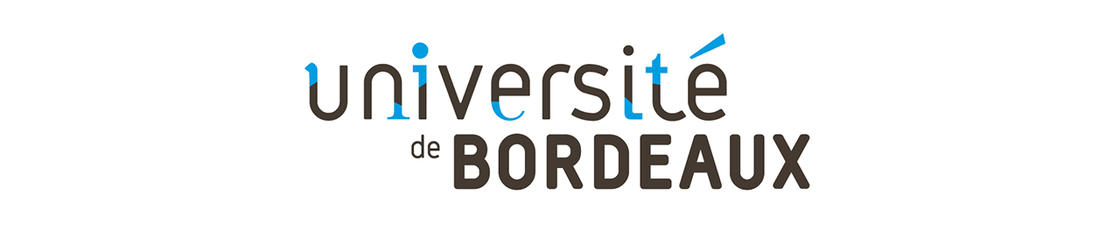
\includegraphics[scale=0.30]{universite-Bordeaux.jpg}~\\[1.5cm]
		\textsc{\LARGE Master 1 Informatique}\\[2cm]
		
		\textsc{\Large Projet de Programmation - Cahier des besoins}\\[1.5cm]
		
		% Titre
		\HRule \\[0.4cm]
		{  \huge{\bfseries Simulation d'écoulement de billes}\\[0.4cm] }
		\HRule \\[2cm]
		
		% Auteurs
		\textsc{GIOVANNANGELI Loann, MAYOLINI Maxime, MOUHOUB Noureddine, RIOU Maxence}\\[0.4cm]
		
		% Bas de page
    	\textsc{\large \today} \\
        \vspace{2cm}
        \textsc{Lien du dépôt : https://services.emi.u-bordeaux.fr/projet/git/pdp-billes/tree/}
	\end{center}
	\end{titlepage}
    
    
%%% PARTIE 0 : RÉSUMÉ %%%
\chapter*{Résumé}

L'objectif de notre projet est de réaliser un simulateur 2D d'écoulement de billes. Il doit être capable de simuler un plateau inclinable, sur lequel il est possible d’ajouter des obstacles en forme de lignes droites et des billes. Son interface graphique doit permettre de pouvoir créer, modifier, paramétrer, exporter, importer et lancer la simulation sur un circuit (l’ensemble plateau-billes-obstacles). Le logiciel doit être muni de son propre moteur physique, gérant l’ensemble des collisions du circuit. \\

Le logiciel réalisé va donc permettre de créer son propre circuit, en choisissant ses dimensions et son inclinaison. Des obstacles et des billes pourront être placés dessus. Puis, l'exécution pourra être lancée, utilisant notre moteur physique et montrant le parcours des billes et leurs interactions avec les différents obstacles jusqu'à leur position finale. L'exécution peut être stoppée à n’importe quel moment. Les circuits sont égalements importables et exportables. De plus, un ensemble de tests (unitaires, de profil et de couverture) sont réalisés sur l’ensemble du projet afin de vérifier que tout fonctionne correctement. 


%%% TABLE DES MATIÈRES %%%
\tableofcontents

%%% PARTIE 1 : INTRODUCTION %%%
\chapter{Introduction}

\section{Moteur physique}

\section{Mécanique du point}

%%% PARTIE 2 : ANALYSE DE L'EXISTANT %%%
\chapter{Analyse de l'existant}

\section{Moteurs physiques}

Un moteur physique est une librairie qui offre un ensemble de fonctionnalités permettant de simuler la physique du monde réel : gravité, chutes, détection de collisions, gestion de collisions, explosions…


\subsection{Moteurs 3D}

Unity est une moteur de jeu multi-plateformes très répandu pour la conception d’applications graphiques 3D. Il intègre le moteur physique PhysX qui permet une simulation en temps réel très réaliste. Pour cela il s’appuie sur l’accélération matérielle des GPU NVIDIA, Unity est très facile d’utilisation : grâce à une interface simple, on peut créer un plan de taille modulable, l’incliner, poser des balles et des obstacles sur ce plan et lancer une simulation. 


\subsection{Moteurs 2D}

Box2D est un moteur physique 2D open source développé en C++ il est également utilisé dans nombreux jeux 2D notamment dans le célèbre jeu pour mobile Angry Birds. Très complet, il détecte et gère les collisions entre des corps rigides de nombreuses formes, les frottements ou encore l’élasticité. il a été porté sur d’autres langages de programmation, comme Java sous le nom de JBox2D.  


\subsection{Limites}

Le problème principal que nous pose ces deux moteurs physiques est qu’ils sont trop complets par rapport à nos besoins. La librairie Box2D comporte beaucoup de fonctions dont nous n’avons aucune utilité dans notre cas et son apprentissage serait trop coûteux en temps. Unity est simple d’utilisation mais se révèle encore plus lourd et nous n’avons pas besoin d’interface graphique 3D, hors c’est son principal intérêt. Par conséquent, les utiliser rendrait notre programme plus lourd inutilement. De plus, ils nous imposent un langage de programmation.

\section{Algorithmes}

\subsection{Détection de collisions}

\subsubsection{Définition d'une collision}

\subsubsection{Optimisations}

\paragraph{QuadTree}

\paragraph{KdTree}

\paragraph{Grid}

\subsection{Résolution de collisions}

\subsubsection{Collision entre deux cercles}

\paragraph{Gestion des forces}

\paragraph{Gestion des masses}

\subsubsection{Collision entre cercle et droite}

%%% PARTIE 3 : ANALYSE DES BESOINS %%%
\chapter{Analyse des besoins}

\section{Besoins fonctionnels}

\subsection{Moteur physique}

L’écoulement des billes dans le circuit doit être simulé par un moteur physique en 2D. On utilisera des combinaisons linéaires pour représenter les déplacements. Pour être réaliste, notre moteur physique doit respecter les lois de la physique terrestre. \\

Notre programme doit gérer le déplacement des billes en prenant en compte la gravité, ainsi que les collisions entre tous les objets du circuit (bille-bille, bille-obstacle). Pour cela nous devons nous baser sur la mécanique du point, notamment le mouvement rectiligne uniformément accéléré. L’accélération de la gravité étant constante. Pour les collisions entre billes nous devons utiliser les équations du choc élastique. 


\subsubsection{Structure des objets}

Dans le circuit, on distingue deux types d’objets : les billes et les obstacles.


\paragraph{Billes}

Le déplacement d’une bille nécessite de connaître sa  position ainsi que sa  vitesse pour calculer sa prochaine position. Sa vitesse est calculée en fonction de l’accélération engendrée par la gravité. La position et le rayon vont servir pour la détection des collisions. Lors d’un choc entre billes, nous devons connaître leur masse et leur vitesse respectives pour répondre aux lois de conversation de la quantité de mouvement et de conservation de l’énergie cinétique. Les billes doivent donc posséder une position, un rayon, une masse et une vitesse dans une certaine direction. 


\paragraph{Obstacles}

Les obstacles sont des segments et sont infranchissables, les billes doivent rebondir dessus. Pour détecter les collisions entre billes et obstacles on doit connaître la position des extrémités du segment. Ces collision sont des chocs inélastiques, l’énergie cinétique de la bille doit diminuer et ainsi que sa vitesse. Il faut donc utiliser un coefficient de restitution inférieur à 1.

\subsubsection{Forces en jeu}

Un moteur physique réaliste prend en compte plusieurs forces : force de gravité, force de réaction (normale) et forces de frottements (air et cinétique). Ces forces sont nécessaires pour le calcul de l’accélération de la bille.

\paragraph{Force de gravité}

La gravité a un impact sur le déplacement des billes, elle les attire vers le bas. La force de gravité est constante : 9,81N. Cette constante est présente dans le calcul de l’accélération de la bille.

\paragraph{Force de réaction}

La force de réaction du plan (circuit) influence sur l’accélération des billes. Plus le plan est vertical (inclinaison proche de 90 degrés), plus la force réaction du plan est faible et donc l’accélération est élevée. Lorsque l’inclinaison est égale à 90 degrés, la force de réaction du plan est nulle et l’accélération est égale à force de la gravité. A l’inverse, si l’inclinaison est de 0 degré, le plan est horizontal et la force de réaction du plan s’oppose parfaitement à la gravité, donc aucune bille ne doit bouger. \\

La force de réaction d’un obstacle est sa normale, qui doit être utilisée pour calculer l’angle de rebond lors d’une collision bille-obstacle. 


\paragraph{Force de frottements}

Pour avoir un roulement des billes, il faut des frottements.  Le moteur physique doit donc prendre en compte les frottements de l’air et les frottements de surfaces (selon matériaux du circuit et des obstacle). L’absence de frottement implique un glissement parfait.

\subsection{Gestion du circuit}

\subsubsection{Billes}

Un circuit doit contenir une liste de billes et permettre l’ajout ou la suppression d’une bille. L’ajout d’une bille ne peut pas se faire si elle va être ajoutée par-dessus un objet déjà existant.

Pour vérifier qu’une bille a bien été ajoutée au circuit, on vérifie qu’elle est bien présente dans la liste de billes du circuits. Il faudra aussi vérifier que l’ajout d’une bille est bien refusé si celle-ci est censée être ajoutée par dessus un objet déjà existant. Pour cela, on ajoutera un objet dans le circuit puis on essaiera d’ajouter une bille aux mêmes coordonnées que l’objet précédent. La liste de billes du circuit ne devra alors pas contenir la bille en question.

\subsubsection{Traces des billes}

Chaque bille du circuit doit contenir une liste de points correspondant à sa trace : ses positions précédentes lors d’une exécution. Cette trace doit être visualisable en temps réel au cours d’une exécution afin de suivre le déplacement des billes.


\subsubsection{Obstacles}

Un circuit doit contenir une liste d’obstacles et permettre l’ajout ou la suppression d’un obstacle. Un obstacle ne doit pas pouvoir être placé par-dessus une bille déjà existante dans le circuit. Par contre, il doit être possible de pouvoir le placer en croisant un autre obstacle.

Pour vérifier qu’un obstacle a bien été ajouté au circuit, on vérifie qu’il est bien présent dans la liste d’obstacles du circuit. Il faudra aussi vérifier que l’ajout d’un obstacle est bien refusé si celui-ci est censé être ajouté par-dessus une bille déjà existante. Pour cela, on ajoutera une bille dans le circuit puis on essaiera d’ajouter un obstacle dont la droite passe par les coordonnées de la bille. La liste d’obstacles du circuit ne devra alors pas contenir l’obstacle en question.


\subsubsection{Réinitialisation}

L’application doit proposer un moyen de suppression de toutes les billes, tous les obstacles ou tous les objets (billes et obstacles).

Pour vérifier que la réinitialisation a fonctionné, on vérifie le contenue des listes d’objets (bille, obstacle ou les deux) qui ont été supprimés.


\subsubsection{Redimensionnement}

L’application doit permettre de modifier la longueur et la largeur du circuit. Si la taille du circuit est réduite, les objets passant hors du circuit doivent être supprimés.

Pour tester que le redimensionnement a fonctionné comme prévu, on vérifie que les nouvelles dimensions du circuit correspondent bien à celles entrées, et on parcourt ses listes de billes et d’obstacles (préalablement remplies) en vérifiant qu’aucun objet ne soit hors du circuit.


\subsubsection{Inclinaison}

L’inclinaison du circuit doit être comprise entre 0 degré et 90 degrés. Elle n’agit que sur un seul axe du circuit. Elle doit pouvoir être modifiée en toutes circonstances (que la simulation soit en cours ou non).

\subsection{Interface graphique}

Afin de permettre une utilisation plus simple et dynamique de l’application, celle-ci devra être utilisable au travers d’une interface graphique.

\subsubsection{Affichage du circuit}

L’interface graphique doit permettre de visualiser l’état du circuit durant toute l’exécution du programme (phase de création de circuit ou phase de simulation d’écoulement de billes).

\subsubsection{Paramétrage du circuit}

L’interface doit permettre de paramétrer le circuit, c’est-à-dire de pouvoir demander à le modifier selon les exigences demandées dans la gestion du circuit, le tout via la souris ou différents boutons.

\subsection{Gestion de l'exécution}

\subsubsection{Démarrer une simulation}

L’application doit permettre de démarrer la simulation d’écoulement des billes. À ce moment, l’utilisateur ne doit plus pouvoir ajouter d’objets au circuit ni le modifier, et les billes doivent être soumises aux différentes forces du moteur physique.

\subsubsection{Mettre en pause une simulation}

L’application doit permettre de mettre en pause une simulation. Les billes ne doivent donc plus bouger, et l’utilisateur peut à nouveau utiliser les fonctionnalités de paramétrage et de création d’objets.

\subsection{Gestion des fichiers}

\subsubsection{Export}

L’application doit permettre de sauvegarder les informations essentielles d’un circuit. On doit donc, a minima, sauvegarder les données du circuit, de chaque obstacle et de chaque bille (avec sa trace).

\subsubsection{Import}

L’application doit permettre de lire un fichier de sauvegarde de circuit et le recréer avec tous ses paramètres : ses dimensions, son inclinaison, ses billes et ses obstacles.

Pour vérifier l’import et l’export, on crée un circuit en mémoire dont on sauvegarde les données et on l’exporte dans un fichier puis on l’importe. Si le circuit résultant de l’import possède les mêmes données que le premier, c’est que l’opération d’export/import a bien sauvegardé et rechargé les données du circuit.


\section{Besoins non-fonctionnels}

\subsection{Performances}

\subsubsection{Temps de chargement}

Le temps de chargement est le temps que doit attendre l’utilisateur après chaque interaction avec l’interface graphique. Ce temps devra être de l’ordre de la seconde.

Pour vérifier que les interactions avec l’interface graphique aient la durée escomptée, on fait un test qui vérifie que la durée de la ou des fonctions mises en œuvre par l’interaction soit inférieure à deux secondes.


\subsubsection{Fluidité de la simulation}

La simulation doit être visuellement réaliste : les billes doivent donner l’impression de glisser et non pas de se téléporter à chaque déplacement.

\subsection{Robustesse du moteur physique}

Il est important que le moteur physique fonctionne correctement afin de garantir le bon comportement des billes. Les tests doivent donc être accentués dessus (plus nombreux et plus robustes).

\subsection{Portabilité}

Afin que l'application soit utilisable par tout utilisateur, l’application doit être multi-plateformes et être exécutable sous Windows, Linux et MacOS.

\section{Besoins optionnels}

\subsection{Interface graphique}

\subsubsection{Zoom}

L’interface graphique est zoomable : l’utilisateur peut choisir d’agrandir visuellement une zone du circuit afin de mieux observer son contenu.

\subsubsection{Paramétrer le coefficient de restitution des obstacles}

L’interface graphique permet de demander la modification du coefficient de restitution d’un obstacle.

\subsection{Fusion de circuits}

L’application permet de fusionner deux circuits, c’est-à-dire les “coller” l’un à côté de l’autre de façon horizontale ou verticale. Les deux circuits à fusionner doivent avoir la même dimension sur le côté où ils sont fusionnés.

\subsection{Modifier la vitesse de simulation}

L’application permet de changer la vitesse d’exécution de la simulation. En outre, on doit avoir l’impression que les billes accélèrent ou décélèrent en fonction de ce facteur.

\subsection{Gestion de fichiers}

\subsubsection{Vidéo de l'exécution}

L’application propose d’enregistrer une simulation puis d’exporter cet enregistrement sous la forme d’un fichier vidéo.

\subsubsection{Impression du circuit}

L’application permet d’imprimer un circuit. L’impression ne prend pas en compte les traces de billes (s’il y en a). Le but est d’avoir une version physique du circuit qui permettrait de reproduire les expériences dans la réalité.

%%% PARTIE 4 : DESCRIPTION DU LOGICIEL %%%
\chapter{Description du logiciel}

\section{Utilisation}

\subsection{Installation}

\subsection{Interface homme-machine}

\subsubsection{Panneau de dessin}

\subsubsection{Panneau de paramétrage}

\subsection{Simulation}

\subsection{Gestion de fichiers}

\subsubsection{Export}

\subsubsection{Import}

\section{Analyse du fonctionnement}

\subsection{Fonctionnement}

\subsubsection{Déplacement des billes}

\paragraph{Gravité}

\paragraph{Événements externes}

\paragraph{Sortie d'écran}

\subsubsection{Collisions}

\paragraph{Gestion}

\subparagraph{Détection}

\subparagraph{Résolution}

\paragraph{Optimisation}

\subsubsection{Traces}

\paragraph{Implémentation}

\paragraph{Affichage}

\subsection{Limites}

\subsubsection{Moteur physique}

\paragraph{Collisions}

\subparagraph{Bugs}

\subparagraph{Mécanique du moteur}

\subsubsection{Interface graphique}

\paragraph{Ergonomie}

\subparagraph{Responsivité}

\subparagraph{Lisibilité}

\paragraph{Taille de circuit}

\paragraph{Méthode d'affichage}

\subparagraph{Bibliothèque d'affichage}

\subparagraph{Gestion de la BufferedImage}

%%% PARTIE 5 : ARCHITECTURE DU LOGICIEL %%%
\chapter{Architecture du logiciel}

\section{Description}

\section{Classes}

%%% PARTIE 6 : TESTS %%%
\chapter{Tests}

\section{Tests unitaires}

\section{Tests de profil}

\section{Test de couverture}

%%% PARTIE 7 : EXTENSIONS %%%
\chapter{Extensions}

\section{Moteur physique}

\subsection{Frottements}

\subsection{Modifier la vitesse de la simulation}

\subsection{Revenir à un pas de temps antérieur}

\section{Interface graphique}

\subsection{Sélection de groupe d'objets}

\subsection{Zoom}

\section{Gestion du circuit}

\subsection{Billes - Coefficient de restitution}

\subsection{Obstacles - Formes}

\section{Gestion de fichiers}

\subsection{Vidéo de l'exécution}

\subsection{Fusion de circuits}

%%% PARTIE 8 : CONCLUSION %%%
\chapter{Conclusion}


\end{document}
